\documentclass{standalone}
\usepackage{tikz}
\usetikzlibrary{calc}
% Add more libraries if required.
\begin{document}
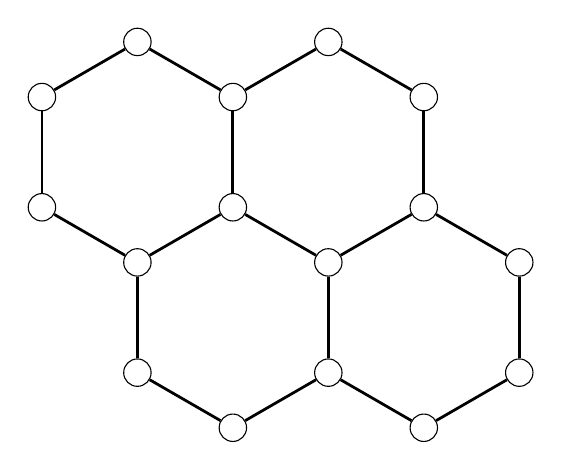
\begin{tikzpicture}[scale=1]
\tikzstyle{every node} = [inner sep=3.5, draw, circle]
\tikzstyle{edge} = [draw, line width=1.0]
\tikzstyle{periedge} = [draw, line width=1.0]
\node[] (-2_1_0) at (-3.637307, 3.500000) {};
\node[] (-1_1_0) at (-1.212436, 3.500000) {};
\node[] (-2_1_1) at (-2.424871, 2.800000) {};
\node[] (-1_-1_1) at (-2.424871, -1.400000) {};
\node[] (-1_1_1) at (0.000000, 2.800000) {};
\node[] (0_0_1) at (1.212436, 0.700000) {};
\node[] (-2_0_1) at (-3.637307, 0.700000) {};
\node[] (1_-1_0) at (1.212436, -0.700000) {};
\node[] (-1_-1_0) at (-3.637307, -0.700000) {};
\node[] (-1_0_1) at (-1.212436, 0.700000) {};
\node[] (0_0_0) at (0.000000, 1.400000) {};
\node[] (0_-1_1) at (0.000000, -1.400000) {};
\node[] (-3_1_1) at (-4.849742, 2.800000) {};
\node[] (-2_0_0) at (-4.849742, 1.400000) {};
\node[] (-1_0_0) at (-2.424871, 1.400000) {};
\node[] (0_-1_0) at (-1.212436, -0.700000) {};
\draw[periedge] (-3_1_1) -- (-2_1_0);
\draw[periedge] (-2_1_1) -- (-1_1_0);
\draw[periedge] (-3_1_1) -- (-2_0_0);
\draw[periedge] (0_0_1) -- (1_-1_0);
\draw[periedge] (-1_1_1) -- (0_0_0);
\draw[edge] (-1_0_1) -- (0_-1_0);
\draw[periedge] (-1_-1_0) -- (-1_-1_1);
\draw[periedge] (-2_1_0) -- (-2_1_1);
\draw[periedge] (0_0_0) -- (0_0_1);
\draw[periedge] (-2_0_0) -- (-2_0_1);
\draw[periedge] (0_-1_1) -- (1_-1_0);
\draw[edge] (-1_0_0) -- (-1_0_1);
\draw[edge] (-2_1_1) -- (-1_0_0);
\draw[edge] (-1_0_1) -- (0_0_0);
\draw[periedge] (0_-1_0) -- (0_-1_1);
\draw[edge] (-2_0_1) -- (-1_0_0);
\draw[periedge] (-1_1_0) -- (-1_1_1);
\draw[periedge] (-2_0_1) -- (-1_-1_0);
\draw[periedge] (-1_-1_1) -- (0_-1_0);
\end{tikzpicture}\end{document}
